%!TEX root = ../main.tex
\section{New Protocol}

%TODO: here we should describe the protocols implemented
%should be rewritten

\iffalse

In this work we implemented a few distributed protocols of the PRF introduced by Boneh et. Al  \cite{darkmatter}:

$PRF_k(x) = R \times (K \times x \mod 2)  \mod 3 $

where $R$ is a randomization matrix in $Z_3$, $K$ is an $m \times n$ key and $x$ is an $n$-length vector. Specifically, we present a new protocol for implementing this PRF. The protocol uses a shared input and output which provides improved performance over the original protocol described in \cite{darkmatter}. For context, we also implement the original protocol \cite{darkmatter} . We also introduce an improved OPRF (Oblivious PRF) protocol, in which one party has the input and one has the key. Below are  details of the protocols.

\subsection{PRF}


\paragraph{notations:} below are the notations we use to describe the protocols: \\
$K$ is the key, represented by an $m \times n$ matrix \\
$x$ is the input, represented by an $n$ size vector \\
$R_x, r_k$ - pre-shared randomness for key $K$ and input $x$ \\
$r$ - random vector in $Z_3$]
We use capital letters for matrices, and $\vec{x}$ notation for vectors \\

\section{Appendix}

\paragraph{Original - Distributed Input Distributed Output (DIDO) - PRF Protocol}

The protocol was introduced in \cite{darkmatter}. The main details of the protocols are described below (\ref{2PartyDarkMatter}). In this setting, both the input and the key are secret shared additively between the two parties. Both the protocol presented in this paper and the original protocol are two-party PRFs. For our implementation, randomization was added in phase 3 to provide $Z_3$ output with 128-bit entropy. 
The protocol is described in \figref{algorithm1}.
%add  a description of the protocol

\begin{figure*}[ht]
	\centering
	\includegraphics[width=1.2\textwidth]{images/old_protocol2.pdf}
	\vspace{-2mm}
	\caption{Old wPRF protocol}
	\label{old_protocol.fig}
	\vspace{-5mm}
\end{figure*}


\begin{algorithm}
	\caption{2-Party dark matter PRF}
	\label{2PartyDarkMatter}
	
	
	Input: ${K_{m\times n} }(i)$ and $\vec{Inp}(i_n)$ key and user input of each user,\\
	$(i = 1...2, n,m = 256)$\\ 
	Output: user 1: $\vec{K} \times x + \vec{r}$\\
	user2: $-  \vec{r}$\\   %SVec = salt vectorx`
	
	\begin{algorithmic}
		
		\STATE \textbf{Preprocessing}:
		
		Output: 	user 1: $\vec{R_a}, \vec{r_b}$ - pre-shared randomness \\
		user 2: $\vec{r_x} $- pre-share randomness \\
		
		\STATE  \textbf{Stage\ 1}: calculate $a \times b \plus c$
		
		input: user 1: ${\vec{A}, \vec{b}, {\vec R_a}, \vec{r_b} } $ \\
		user 2: ${\vec{x}, \vec{r_x},  \vec{z} }$ \\
		
		\begin{enumerate}
			
			\item user 2 $\vec{m_x} = \vec{x} -\vec{r_x}  \rightarrow  $  user 1
			
			\item user 1  $ \leftarrow   \vec{M_a} =  \vec{A} - \vec{r_A}   $ user 2
			
			\item user 2 $ \vec{m_b} = \vec{R_a} \times \vec{m_x} + \vec{b}  - \vec{r_b}  \rightarrow $ user 1
		\end{enumerate}
		
		Output: $user 1: \vec{- b} $  \\
		$user 2: \vec{M_a} \times \vec{x} + \vec{m_b} + \vec{z} = \vec{A} \vec{x} + \vec{b}$ \\
		
		\STATE  \textbf{Stage\ 2}: Oblivious Transfer
		input: 	 user 1:  $\vec{r_1}, \vec{r_2}, \vec{r_a}, \vec{r_b}$ - vectors in $Z_3$
		user 2:  $\vec{x}, \vec{r_x}$ - vectors in $Z_2$, $\vec{z} $ - vector in $Z_3$
		
		
		\begin{enumerate}
			\item user 1  $ \leftarrow   \vec{m_x} = \vec{x} \oplus \vec{r_x}$   user 2
			
			\item user 1:  $  \vec{m_1} = \vec(- m_x)  \vec{r_a} + \vec{m_x} \vec{r_b} + \vec{r_1}   \rightarrow $   user 2
			
			\item user 1:  $  \vec{m_2} = \vec(m_x)  \vec{r_a} + \vec{- m_x} \vec{r_b} + \vec{r_2}  \rightarrow $   user 2
			
			
		\end{enumerate}
		
		output:  user 2: $\vec{w}:= \vec{x} \times \vec{m_2}+ - \vec{x}  \times \vec{m_1} - \vec{z}$
		
		
		\STATE  \textbf{stage 3}: $Z_3$ randomization  
		
	\end{algorithmic}
	
\end{algorithm}




%add table with parameters, including communication

\paragraph{Our improved (DIDO) PRF protocol}

\begin{figure*}[ht]
	\centering
	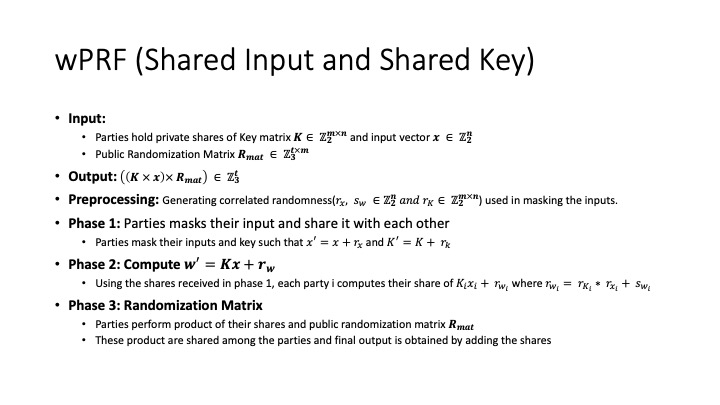
\includegraphics[width=0.8\textwidth]{images/sisk.jpg}
	\vspace{-2mm}
	\caption{Distributed Input Distributed Output wPRF protocol}
	\label{sisk.fig}
	\vspace{-5mm}
\end{figure*}

\begin{algorithm}
	\caption{2-Party Distributed PRF (Shared input and Shared Key)}
	\begin{algorithmic}
		\STATE Input: $x \in \mathbb{Z}_{2}^{n}$
		\STATE Key: $K \in \mathbb{Z}_{2}^{m \times n}$
		\STATE Output: $y \in \mathbb{Z}_{3}^{t}$
		\STATE Preprocessing: Generate correlated randomness $r_{x}, s_{w} \in \mathbb{Z}_{2}^{n}. and R_{k} \in \mathbb{Z}_{2}^{m \times n}$\\
		and compute $ r_{w} = R_{k} \cdot r_{x} \oplus s_{w}$
		
		\STATE Stage 1: Mask the inputs: Both the parties mask their shares of input and key they hold and the mask are shared.\\
		$K_{i}^{\textrm'} = K_{i} + Rk_{i}$ and 
		$x_{i}^{\textrm'} = x_{i} + rx_{i}$ and 
		
		
		\STATE Stage 2: Merging the shares, each party computes $w^{\textrm'} = K \times x + rw$. This is done as follows\\
		
		
		\STATE stage 3: $Z_3$ randomization  
		
	\end{algorithmic}
\end{algorithm}



%add  a description of the protocol

%add table with parameters, including communication

\subsection{OPRF}
This is a new OPRF protocol, which improved the performance over the original OPRF protocol descirbed in \cite{darkmatter}. In this setting, one party has the input and another party has the key.

\begin{figure*}[ht]
	\centering
	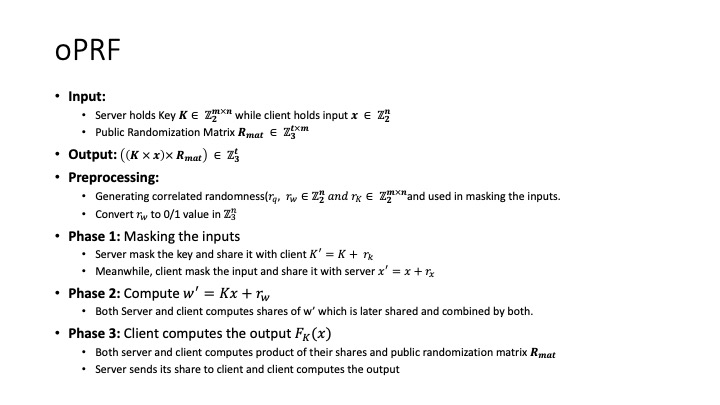
\includegraphics[width=0.8\textwidth]{images/oprf.jpg}
	\vspace{-2mm}
	\caption{oPRF protocol}
	\label{oprf.fig}
	\vspace{-5mm}
\end{figure*}


\begin{algorithm}
	\caption{2-Party oPRF}
	\begin{algorithmic}
		
		\STATE Preprocessing
		
		\STATE Stage\ 1: calculate $a \times b \plus c$
		
		\STATE Stage\ 2: Oblivious Transfer
		
		\STATE stage 3: $Z_3$ randomization  
		
	\end{algorithmic}
\end{algorithm}

\fi


\section{Implementation}
\label{sec:technical_overview}



%%%%%%%%%%%%%%%%%%%%%%%%%%%%%%%%%%%%%%%%%%%%%%%%%


\subsection{Parameters}
The input variable to the PRF functions are the key $K$ which is of size $m \times n$ and each input is a vector of size $n$. 
To save storage space, the key was implemented as a Toeplitz matrix, requiring $2 \cdot n$ bits of storage space.
In phase 3 of the algorithm, a randomization matrix is used which is of size $r \times n = 81 \times 256$, resulting in entropy of 128 bits.

\subsection{representing $Z_2$ vector}

Bit slicing: this bit-wise packing technique was used to optimize the run-time, each 64 bits were represented by a word. Since each key is of size $m \times n$ and each input is a vactor of size $n$, it is possible to pack each 64 rows into $m$ words. This may result in time saving of up to $\times 64$ of the run-time.

\subsection{Representing $Z_3$ vector}

To optimize the randomization in $Z_3$, which requires a matrix-vector multiplication in the last phase of the PRF calculation, we implement two optimization methods:

\subsubsection{Bit slicing and operations:} this was done by representing a vector over $Z_3$  as two binary vectors - one LSB's and one MSB's. 

The Addition, subtraction, multiplication and MUX mod 3 were implemented using the protocols defined in table ref{tab:multicol}. One of the properties that were utilized to implement this was:\\
mult-by-2 $\mod 3  \leftrightarrow$ negation $ \mod 3 \leftrightarrow$ swap the MSB and LSB\\

Such a vector is sometimes being represented as a vector of $2 \times n$ bits. One example is when this vector is sent as an input to the Oblivious Transfer mechanism. 
The algorithms can be found in ~\cref{alg:algpack1,alg:algpack2,alg:algpack3,alg:algpack4}.

% TODO: replace with a table - COMPLETED

input:   $\vec{l_1}, {m_1}$ - LSB and MSB vectors of value 1  \\
					${l_2}, {m_2}$ - LSB and MSB vectors of value 2
					${s}$ - binary select vector

\begin{table}[ht]
\caption{Operations in $Z_3$}
\begin{center}
\begin{tabular}{|c|l|}
    \hline
    \textbf{Operations} & \textbf{Methods}\\
    \hline
    \multirow{3}{*}{Addition} & ${t} := ({l_1 \wedge m_2}) \oplus ({l_2 \wedge m_1})$\\
    & $m_{\mathrm{out}} := ( l_1 \wedge  l_2 ) \oplus  t $ \\
    & $l_{\mathrm{out}} :=m_1 \wedge m_2 ) \oplus t $ \\
    \hline
    \multirow{3}{*}{Subtraction} & ${t} := ({l_1} \wedge {l_2}) \oplus ({m_2} \wedge {m_1})$;\\
    & $m_{\mathrm{out}} := (l_1 \wedge m_2 ) \oplus t$;\\
    & $l_{\mathrm{out}} := (m_1 \wedge l_2 ) \oplus t$; \\
    \hline
\multirow{3}{*}{Multiplication} & $m_{\mathrm{out}}:= (l_1 \vee m_2) \wedge   (m_1 \vee l_2)$; \\
    & $l_{\mathrm{out}} := (l_1 \vee l_2) \wedge     (m_1 \vee m_2)$;\\
    \hline
\multirow{3}{*}{MUX} & $m_{\mathrm{out}} :=( m_2 \vee s) \wedge (m_1 \vee (- s) )$; \\
    & $l_{\mathrm{out}}[i] :=( l_2 \vee s) \wedge (l_1 \vee (- s) )$; \\
    \hline

\end{tabular}
\end{center}
\label{tab:multicol}
\end{table}

%======================================
\iffalse%Start of comment
\begin{algorithm}
	\caption{Addition in $Z_3$}
		\label{alg:algpack1}  Item 1:
		input: $\vec{l_1}, \vec{m_1}$ - LSB and MSB vectors of value 1  \\
		  	  	$\vec{l_2}, \vec{m_2}$ - LSB and MSB vectors of value 2
		
\begin{enumerate}

	\item $\vec{T} = (\vec{l_1} \BitOr \vec{m_2}) \oplus (\vec{l_2} \BitOr \vec{m_1})$;
	\item $MSB_{res} = ( \vec{l_1} \BitOr \vec{l_2} ) \oplus  \vec{T} $;
	\item $LSB_{res} = (\vec{m_1} \BitOr \vec{m_2} ) \oplus \vec{T} $;
	
	\end{enumerate}
	
\end{algorithm}

\begin{algorithm}
		\caption{Subtraction in $Z_3$}
		\label{alg:algpack2} Item 2:

	
		input: $\vec{l_1}, \vec{m_1}$ - LSB and LSB vectors of value 1  \\
                  $\vec{l_2}, \vec{m_2}$ - LSB and LSB vectors of value 2
                  
\begin{enumerate}

	\item $\vec{T} = (\vec{l_1} | \vec{l_2}) \land (\vec{m_2} | \vec{m_1})$;
	\item $MSB_{res} = (\vec{l_1} | \vec{m_2} ) \land \vec{T}$;
    \item $LSB_{res} = (\vec{m_1} | \vec{l_2} ) \land \vec{T}$;
\end{enumerate}
	
	\end{algorithm}



\begin{algorithm}
			\caption{Multiplication of two trinary vectors $Z_3$}
		\label{alg:algpack3} Item 3:

		
				input: $\vec{l_1}, \vec{m_1}$ - LSB and LSB vectors of value 1  \\
		$\vec{l_2}, \vec{m_2}$ - LSB and LSB vectors of value 2
		
			\begin{enumerate}
	\item  $\vec{LSB_{res}} = ((\vec{l_1} \BitAnd (\vec{l_2}) \land     ((\vec{m_1} \BitAnd (\vec{m_2})       $
	\item	$\vec{MSB_{res}}= ((\vec{l_1} \BitAnd (\vec{m_2}) \land     ((\vec{m_1} \BitAnd (\vec{l_2})       $

	\end{enumerate}
		
	\end{algorithm}

\begin{algorithm}
		\caption{MUX implementation of two trinary vectors $Z_3$}
			\label{alg:algpack4} 

	
		input:   $\vec{l_1}, \vec{m_1}$ - LSB and LSB vectors of value 1  \\
					$\vec{l_2}, \vec{m_2}$ - LSB and LSB vectors of value 2
					$\vec{select}$ - binary vector

	\begin{enumerate}
		\item for each word $i$
	    \item $\vec{LSB[i]} =( \vec{l_2} \land \vec{s[i]}) | (\vec{l_1} \land \vec{- s[i]})$
	    		    \item $\vec{MSB[i]} =( \vec{m_2} \land \vec{s[i]}) | (\vec{m_1} \land \vec{- s[i]})$
		
	\end{enumerate}
	
\end{algorithm}

\fi%END of comment

\subsubsection{Integer packing and operations:} As an alternative to bit splicing, integer packing was explored. Since each number is a trinary number, the multiplication of each row by the output vector can be any number between -256 to 256. To explore this option, we represented each number by 9 bits, and packed 7 numbers into each word. This was expected to result in time saving of up to $\times 7$. Testing this option indeed proved to be significantly slower than the first method of packing. We therefore continued using the first packing method of packing instead.
Note: since each trinary number can be either 0,1 or 2, we can add up to 255 numbers and never exceed 511. Moreover, if we take a random sample, we can add 256 numbers and the probability of carryover is negligible. We use this to multiply a packed trinary vector with a ternary matrix with 256 columns (see algorithm below).
	
	$x_0 \dots x_6 \epsilon Z_3 = {0,1,2}$
	
	$ \rightarrow x = \sum_{i=0}^{6} (512^i) \times c_i, x_i \epsilon [0 ... (2^(64)-1)]$


%TODO: IS THIS CORRECT? CHECK AND CORRECT

\paragraph{Matrix multiplication - using a lookup table: }
List of things to be written\\

%\textbf{Comment 1: What is lookup table, explain with context?}\\
%\textbf{Comment 2: Why is it required and what does it replace, are there any advantage}\\
%\textbf{Comment 3: How does it work, please explain with a diagram, if possible}\\
%\textbf{Comment 4: What are the disadvantage(s) of having/using a lookup table}\\ \\ \\ 

\iffalse
\begin{figure*}[ht]
	\centering
	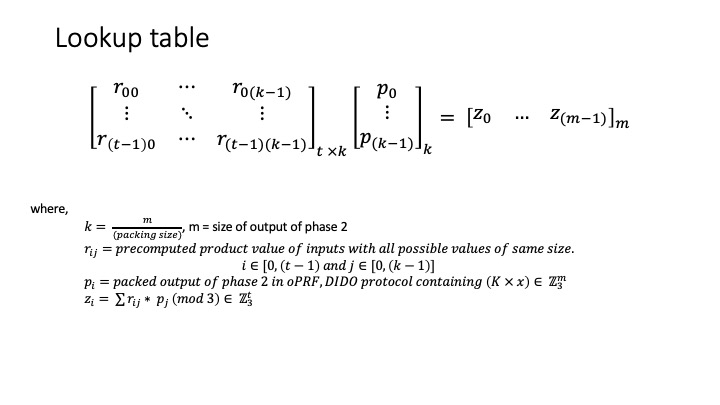
\includegraphics[width=0.8\textwidth]{images/lookup.jpg}
	\vspace{-2mm}
	\caption{Use of lookup table in phase 3}
	\label{oprf.fig}
	\vspace{-5mm}
\end{figure*}

\fi

Phase 2 of the protocols(DIDO, oPRF) outputs m bits $\in \mathbb{Z}_2$. Phase 3 takes output of phase 2 and performs a matrix vector multiplication with a public randomization matrix $Rmat \in \mathbb{Z}_{3}^{t \times m} $ to output $\mathbb{Z}_{3}^{t} $\\
Naive method of performing this matrix-vector multiplication will be to multiply and add individual bits, which will take a long time. An optimized and faster version was also implemented as a function using packed bits. This packed version of multiplication runs way faster than the naive implementation. In order to further optimize the run-time, a lookup table is used to perform the task.\\

Lookup table is a matrix whose elements are precomputed product value of packed inputs(output of phase 2) with all possible combinations of similar sized packed values. Suppose, if inputs are packed as a 8-bit word, the matrix will contain all possible combination of product of 8-bit input and all values from 0 to $2^{8}-1$. \\

Implementing protocol using the lookup method consists of two substages in phase 3:\\
\begin{itemize}
	\item{\textbf{Preprocessing Stage: } Creation of lookup table}
	\item{\textbf{Multiplication Stage: } Usage of lookup table}
\end{itemize}


The prime advantage of replacing matrix vector multiplication with lookup table is speed improvement. This is due to creation of lookup table at the preprocessing stage of the protocol. While creation of a lookup table takes a prolong period of time, the multiplication stage is as simple as accessing an element from a matrix. This speeds up the last stage of the protocol, hence significantly improving the overall speed of execution.


To this end, the randomization matrix is assumed to be constant and divided into 16 matrices of size $81 \times 16$. A lookup table of size $16 \times 2^{16}$ is created during the pre-processing stage. During runtime, the input is divided to MSB and LSB, and each consecutive 16 bits (16 rows in the matrix) are used as separate input to the lookup table.  Similarly, we explored dividing the table into 8 matrices of size $81 \times 32$, resulting in a lookup table of size $8  \times 2^{32} $. However, due to the large table size, this crashed the system during runtime and we were not able to get results for it.	

There are two challenges of using a lookup table as compared to matrix-vector multiplication
\begin{itemize}
	\item{Huge storage requirement/ more time in preprocessing}
	\item{Find a perfect value that can balance between less storage and speedy lookup: Finding }
\end{itemize}

\subsection{Putting it all together}

\begin{itemize}
	\item{\textbf{Implemented DIDO protocol was 50.7\% faster and oPRF was 54\% than implemented wPRF protocol described in TCC'18.}}
	\item{\textbf{Using lookup table, the speed increase was significant at 70\% and 76.5\% for DIDO and oPRF respectively.}}
\end{itemize}

\section{Analysis}

Table \ref{CommunicationCosts} includes the computation and communication results for the different protocol.

%New Communication Cost
\begin{table}[htbp]
	\label{CommunicationCosts}
	%[h]
	\begin{center}
		%\begin{minipage}{10cm}
		\begin{tabular}{|c|c|c|c|c|}
			\hline
			\textbf{Protocol} & \textbf{Rounds}  & \textbf{Message Counts} &  \textbf{Preprocessing Size} & \textbf{Comm Costs}  \\
			\hline
			\hline
			\textbf{Old Protocol}  & 4  & 11 & 8n & $(6n+3m+2t)$ \\
			\hline
			\textbf{DIDO PRF protocol} & 2	& 8 & (2s+m)/(4n+7m) & $(4n+2m+2t)$  	\\
			\hline
			\textbf{OPRF} & 3 & 5 & - &  $(2n+2m+t) bits$	\\
			\hline
			\textbf{Discrete log-based PRF} &  - & - &  & \\
			\hline
			
		\end{tabular}
		
		\vspace{-1mm}
		\caption{Communication Analysis of different protocols}
		\label{CommunicationCosts}
		%\end{minipage}
	\end{center}
	\vspace{-5mm}
\end{table}


\section{Benchmarking}

We compare our run-time to discrete-log based PRFs. To this end, we use the lib sodium library \cite{LibSodium}. The library uses elliptic curve 252 bits, and includes a function that performs scalar multiplication ('crypto\_scalarmult\_ed25519').


\section{Experimental Results}

The system was tested using Ubuntu Server 18.04 on a t2.medium AWS environment. To record the timings, the code was run in a loop 1000 times. Below are run-time results for running a single instance of PRF in microsecond. The results include both centralized and distributed versions of the PRF. In order to increase efficiency, packing and lookup tables were used. The packing indicates both the $Z_2$ and $Z_3$ packing.

%add table
\begin{table}[htbp]
	%[h]
	\begin{center}
		%\begin{minipage}{10cm}
		\begin{tabular}{|c|c|c|c|c|c|}
			\hline
			\textbf{Protocol} & \textbf{Packed }  &  \textbf{lookup} & \textbf{Rounds/sec} & Runtime($\mu$ sec) & Computation\\
			\hline
			\hline
			\textbf{Centralized weak PRF}  & N  & N  &  50K&	20.2 & -\\
			\hline
			\textbf{Centralized weak PRF} & Y  &  N & 65.4K &	18.5 & 70n \\
			\hline
			\textbf{Centralized weak PRF} & Y  &  Y & 165K &6.08 & 34n\\
			\hline
			\textbf{Original distributed dark matter} & Y & N &  24K & 40.56	&210n \\
			\hline
			\textbf{DIDO} & Y & N & 49K &  20.20& 193n\\
			\hline
			\textbf{DIDO} & Y & Y & 82K &  12.12& 133n\\
			\hline
			\textbf{oPRF} & Y & N & 53K &  18.66& 135n\\
			\hline
			\textbf{oPRF} & Y & Y & 104K &  9.52& 76n \\
			\hline
			\textbf{Discrete log-based PRF} &  - & - & 35K & 28.69 &-\\
			\hline
			
		\end{tabular}
		
		\vspace{-1mm}
		\caption{Run-time of different protocols}
		\label{RuntimeTable}
		%\end{minipage}
	\end{center}
	\vspace{-5mm}
\end{table}







